%! Author = jonathan
%! Date = 5/27/25
\chapter{FP16 Memory Throughput}\label{ch:fp16-memory-throughput}
\begin{figure}[!ht]
    \centering
    \begin{subfigure}{\textwidth}
        \centering
        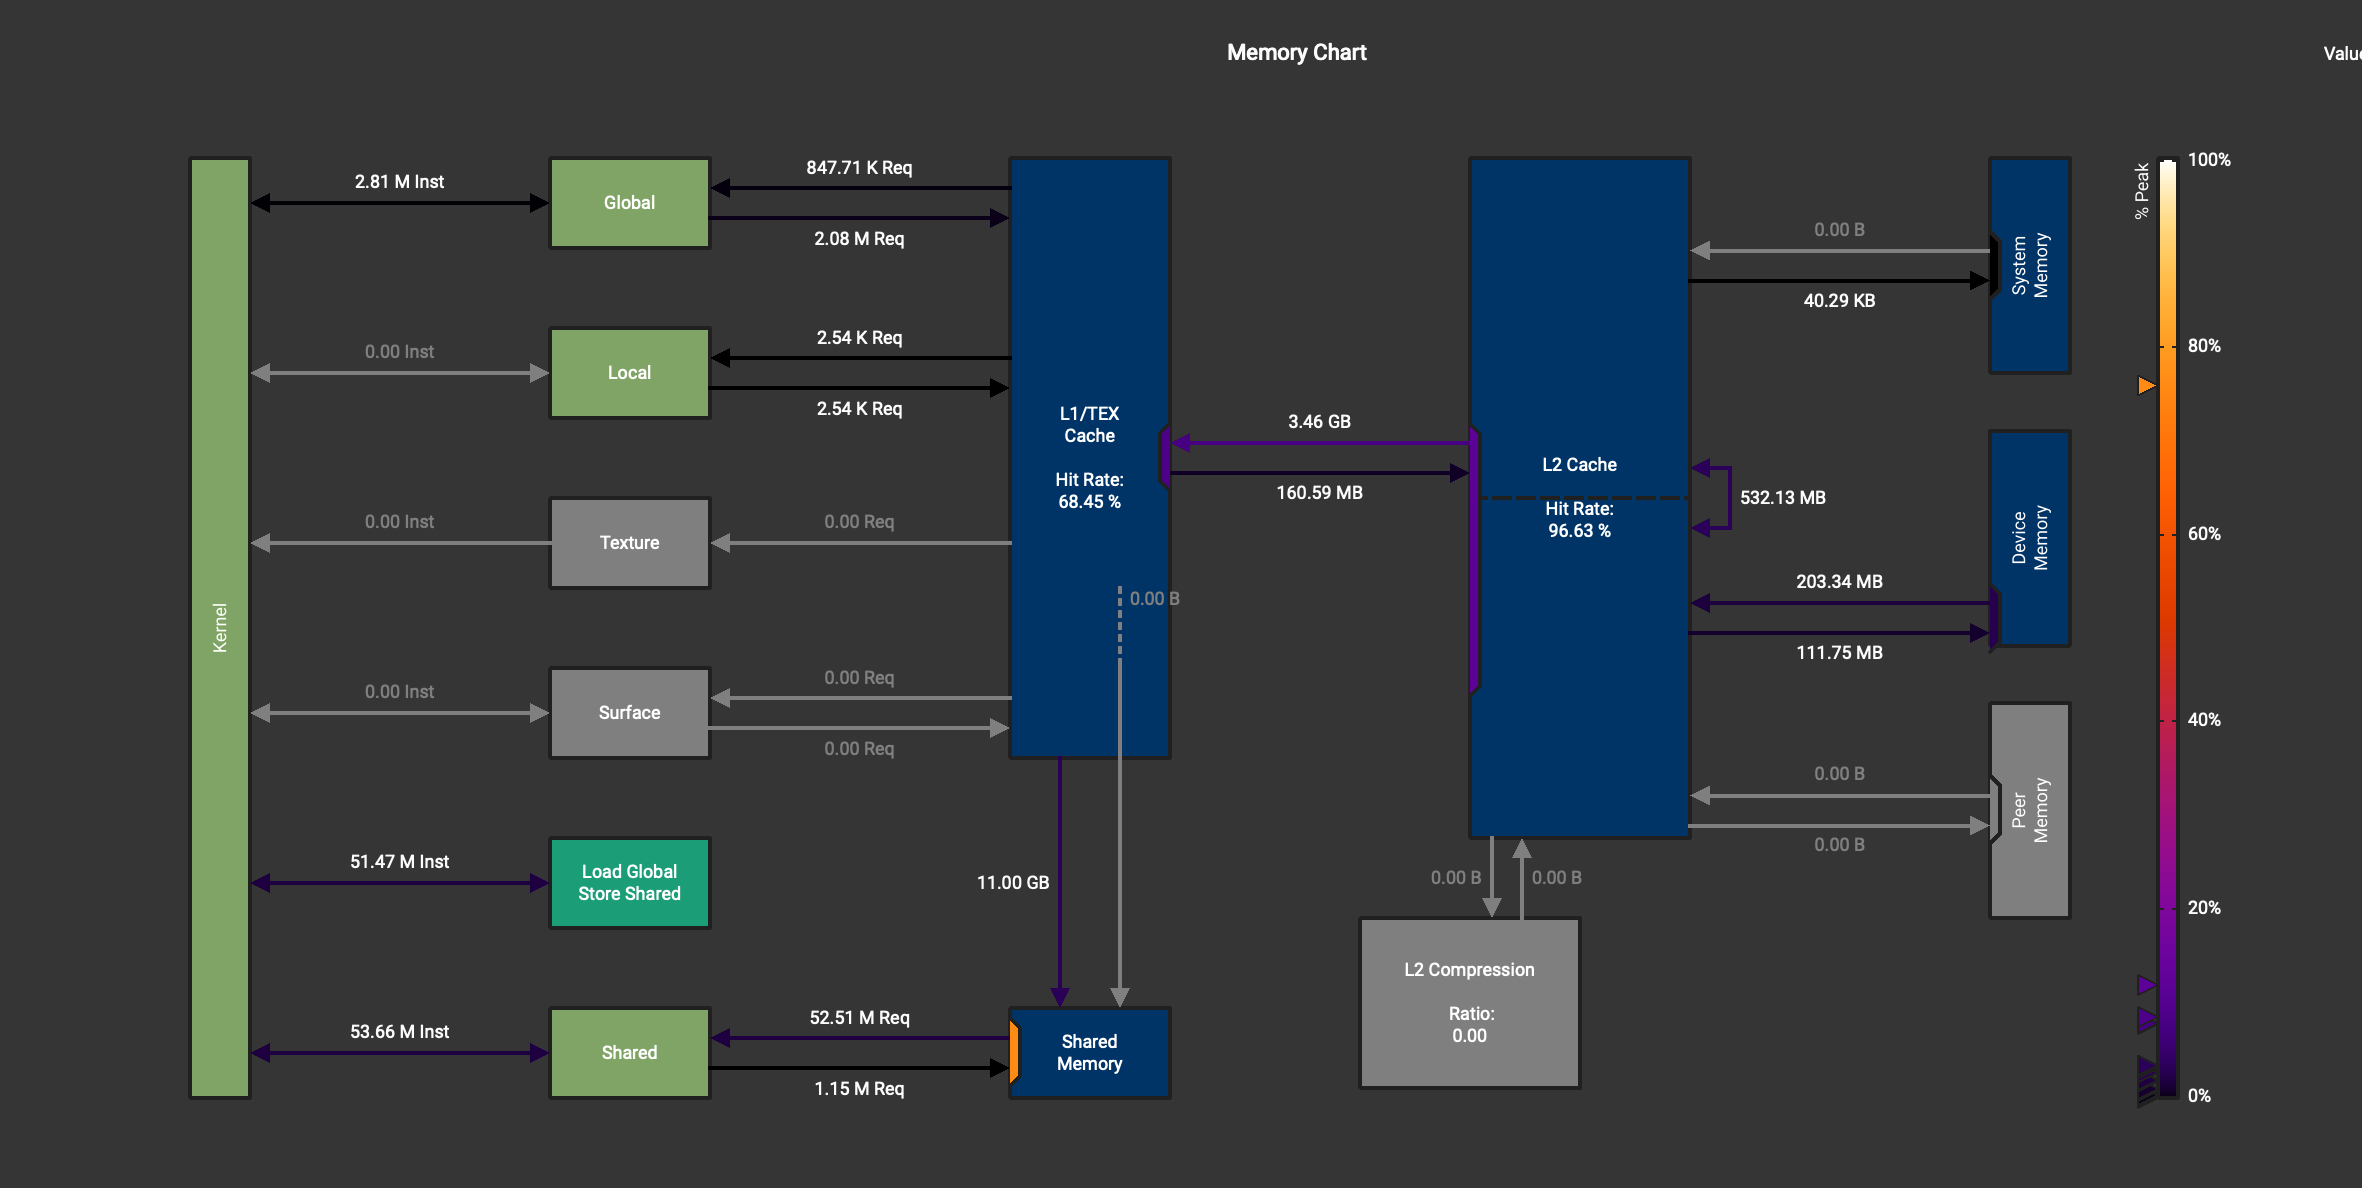
\includegraphics[width=0.9\linewidth, keepaspectratio]{figures/fp16_t}
        \caption{Memory subsystem throughput for FP16}
        \label{sub:fp16}
    \end{subfigure}
    \hfill
    \begin{subfigure}{\textwidth}
        \centering
        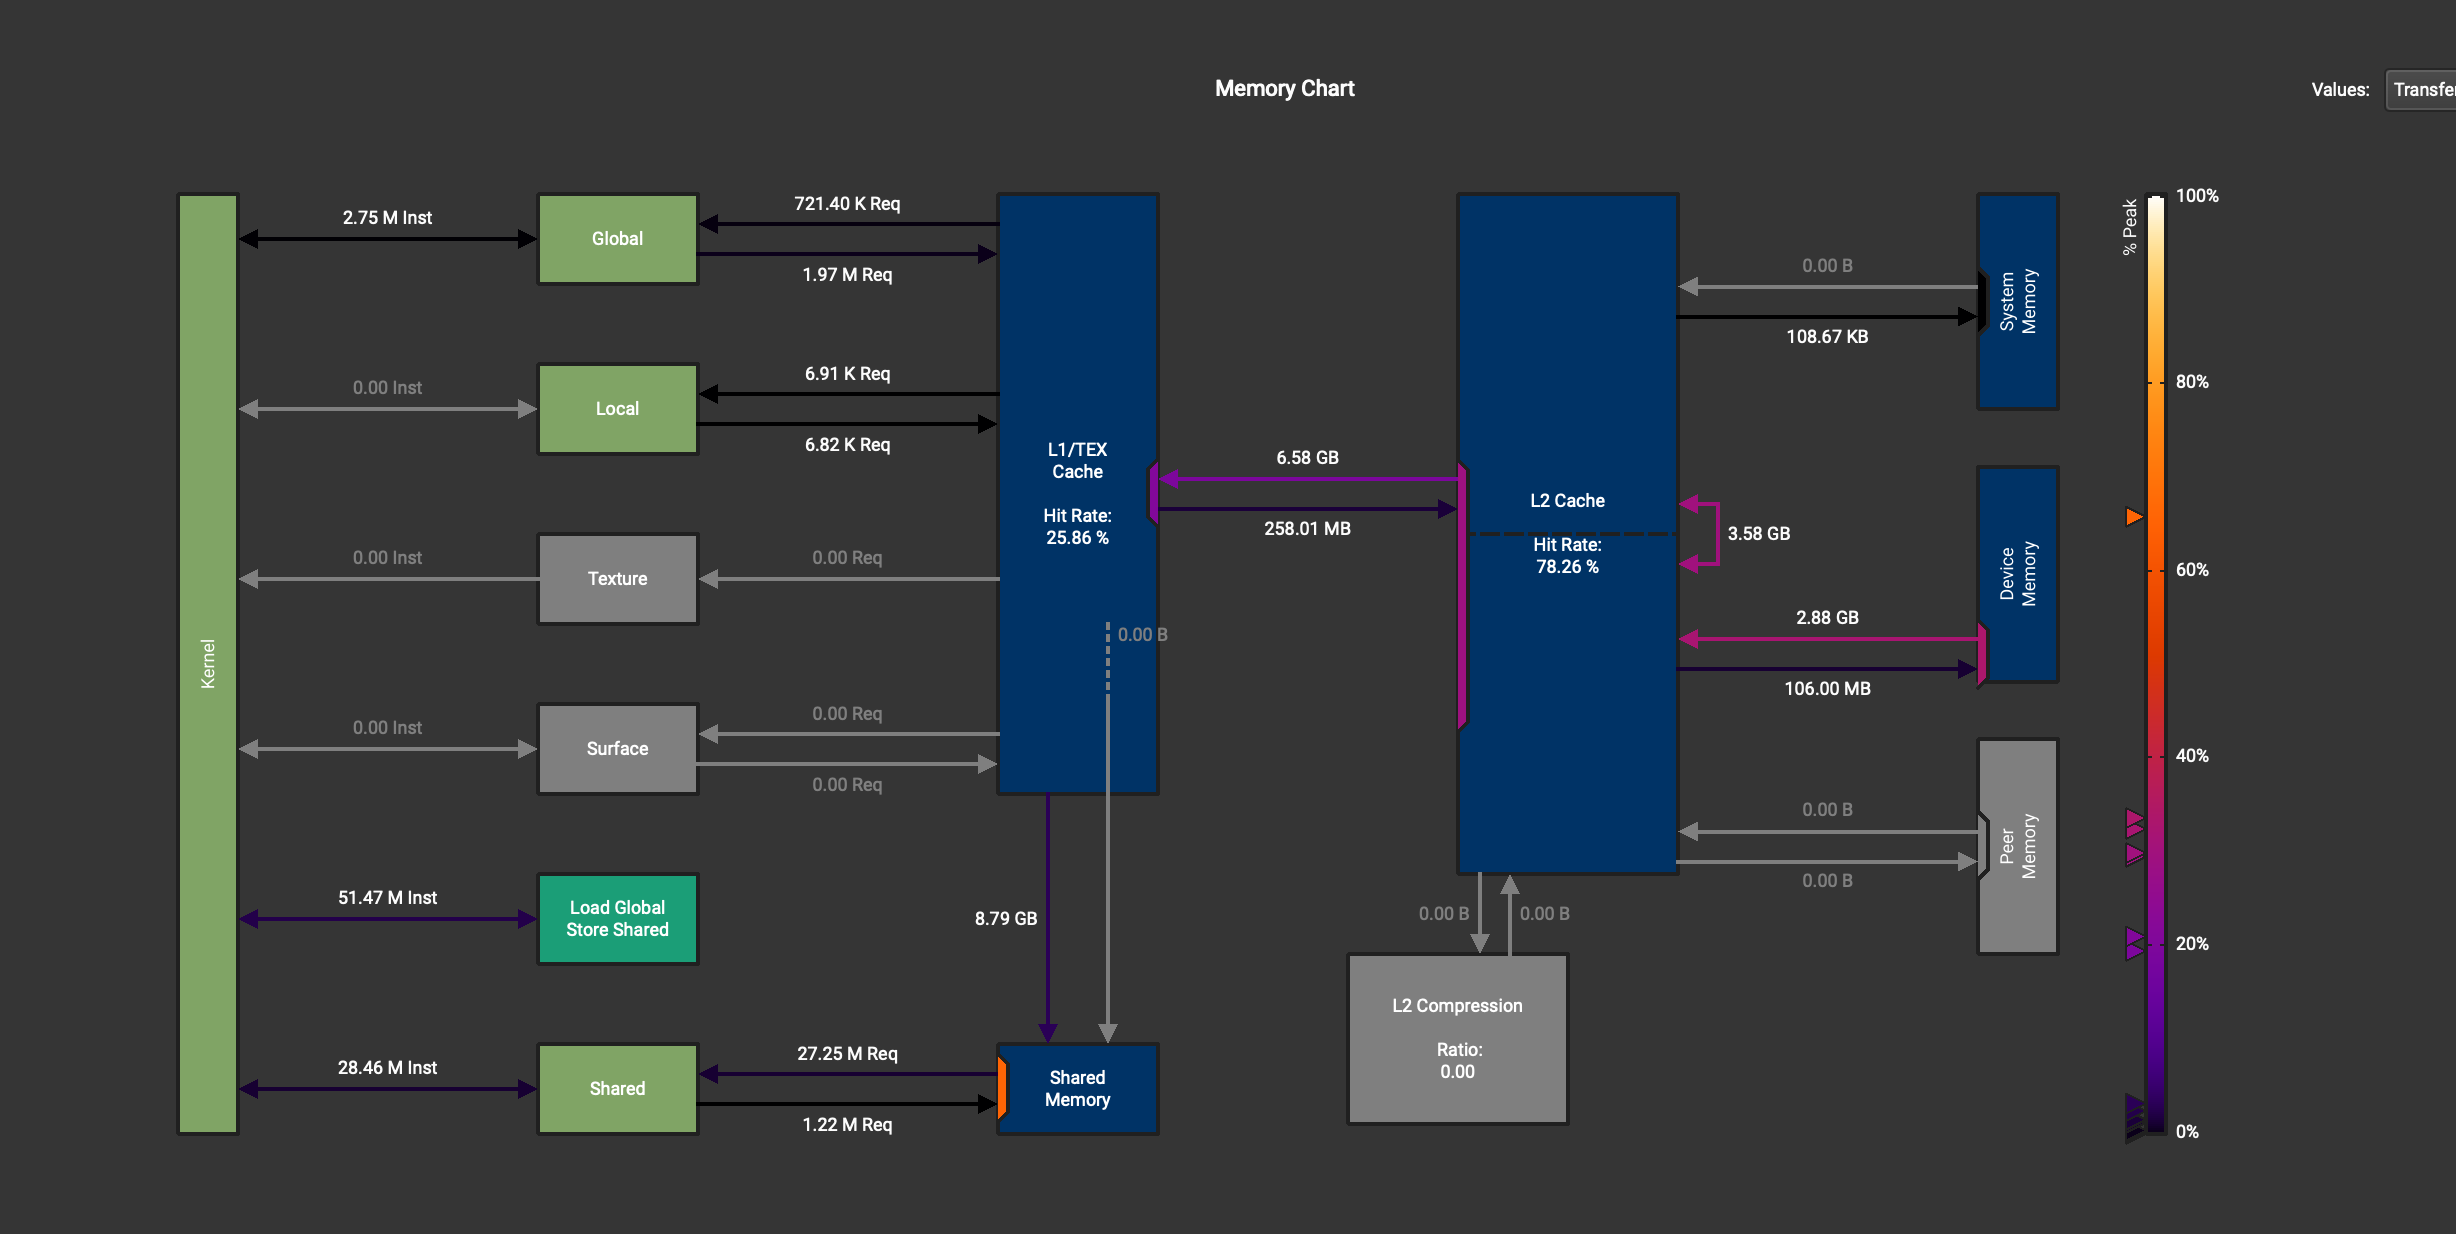
\includegraphics[width=0.9\linewidth, keepaspectratio]{figures/fp32_t}
        \caption{Memory subsystem throughput for FP32}
        \label{sub:fp32}
    \end{subfigure}
    \caption{Here, we report the total GPU memory throughput for both FP16 (top) and FP32 (bottom) variants of \sysname.
    Notably, the FP16 implementation issues approximately $2\times$
        more shared memory instructions compared to its FP32 counterpart
        under identical workloads.
        We attribute this inefficiency to
        suboptimal shared memory layouts in \sysname when
        operating on half-precision data.
        While this bottleneck is addressable through improved layout strategies,
        we leave its resolution to future work due to time constraints.}
    \label{fig:mem_t}
\end{figure}